\documentclass{article}

\usepackage{tikz}

\title{Counting Set A}
\date{}
\author{}

\begin{document}
\maketitle
\noindent Problems should be solved without calculators unless otherwise 
specified. Remember to explain how you solved a problem.
\begin{enumerate}
    \item In how many ways can the letters $A$, $B$, $C$, and $D$ be 
        arranged so that no letter is adjacent to any letter that comes 
        immediately before it or immediately after it alphabetically?
        \vspace{3cm}
    \item If there are $3$ boys and $4$ girls in a group and two are chosen 
        to give a report, what is the probability that one boy and one girl 
        are chosen?
        \vspace{3cm}
    \item Cedric has four times as many shirts and pants, and he can use 
        them to make $100$ different shirt-and-pants outfits. How many pants 
        does Cedric have?
        \vspace{3cm}
    \item How many rectangles (of any size) are there in this figure?
        \begin{center}
            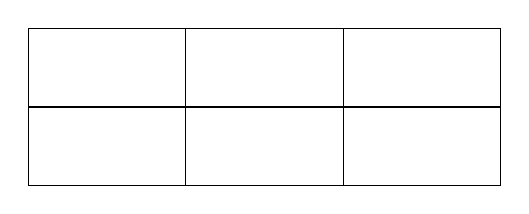
\begin{tikzpicture}
                \draw (0, 0) -- (6, 0) -- (6, 2) -- (0, 2) -- cycle;
                \draw (0, 1) -- (6, 1);
                \draw (2, 0) -- (2, 2);
                \draw (4, 0) -- (4, 2);
            \end{tikzpicture}
        \end{center}
        \vspace{3cm}
    \item Every student who applied for admission to a veterinary school has 
        at least one pet: $30$ have a cat, $28$ have a dog, and $26$ have 
        fish. If $13$ students have a fish and a cat, $15$ students have 
        fish and a dog, $11$ students have both a cat and a dog, and $4$ 
        students have a cat, a dog, and a fish, how many students applied to 
        veterinary school? Hint 1: Use this Venn diagram. Hint 2: The 
        inclusion-exclusion principle can be used for more than two sets. If we 
        added the number of people who have a cat, the number of people who have 
        a fish, and the number of people who have a dog together, how many times 
        is each region in the Venn diagram counted? What can we subtract in 
        order to correct for regions being counted multiple times? What might we 
        need to add back in order to ensure all regions are counted? Try looking 
        up the inclusion-exclusion principle for more hints.
        \begin{center}
            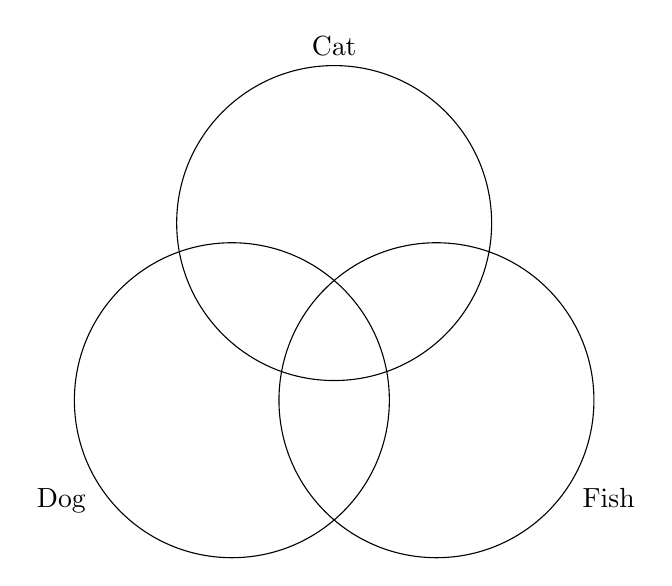
\begin{tikzpicture}
                \draw (90 : 1.5) circle (2);
                \node[above] at (90 : 3.5) {Cat};
                \draw (210 : 1.5) circle (2);
                \node[below left] at (210 : 3.5) {Dog};
                \draw (330 : 1.5) circle (2);
                \node[below right] at (330 : 3.5) {Fish};
            \end{tikzpicture}
        \end{center}
        \vspace{3cm}
\end{enumerate}
\end{document}
